% =============================================================================
% Methodology Section — Overleaf-compatible LaTeX
% Required packages (add to preamble):
%   \usepackage{booktabs, graphicx, amsmath, amssymb, multirow, caption, subcaption}
% Assumes figures are uploaded to a figures/ directory in the Overleaf project.
% =============================================================================

\section{Methodology}
\label{sec:methodology}

%%%%%%%%%%%%%%%%%%%%%%%%%%%%%%%%%%%%%%%%%%%%%%%%%%%%%%%%%%%%%%%%%%%%%%%%%%%%%%%%
\subsection{Problem Framing}
\label{subsec:problem_framing}

\paragraph{Target variable.}
The target variable is the hourly total electricity grid load for the Netherlands, measured in megawatts (MW) and sourced from the European Network of Transmission System Operators for Electricity (ENTSO-E)~\cite{entsoe_power_stats}. This represents the aggregate demand on the Dutch transmission system operated by TenneT, including both onshore consumption and offshore wind farms connected to the national grid. The dataset spans January~2012 to December~2025, comprising 122,736~hourly records with near-complete coverage (0.01\% null, corresponding to 13~hours of DST transition gaps).

\paragraph{Forecasting horizons.}
Following established Dutch grid load forecasting literature~\cite{curiel_integrating_2025, ashtar_hybrid_2025, van_de_sande_enhancing_2024}, we evaluate three direct multi-step forecasting horizons:
\begin{itemize}
    \item $H_{\text{pred}} = 168$~h (1~week) — operational dispatch and scheduling,
    \item $H_{\text{pred}} = 720$~h ($\sim$1~month) — capacity planning and maintenance,
    \item $H_{\text{pred}} = 1{,}440$~h ($\sim$2~months) — medium-term grid adequacy assessment.
\end{itemize}
These horizons span short-to-medium-term planning windows that are operationally relevant to Dutch grid operators and enable direct comparison with results reported by van de~Sande et~al.~\cite{van_de_sande_enhancing_2024} ($r = 0.93$ at 180~days), Ashtar et~al.~\cite{ashtar_hybrid_2025} (MAPE 1.88\% at 180~days), and Curi\"el et~al.~\cite{curiel_integrating_2025}. In contrast to the NTL-based studies by Chen et~al.~\cite{chen_monthly_2025} (monthly), R.~et~al.~\cite{r_forecasting_2025} (daily), and Borunda et~al.~\cite{borunda_machine_2025} (annual), our hourly granularity captures diurnal and intra-week patterns that are invisible at coarser temporal resolutions.

\paragraph{Lookback window.}
At prediction time~$t$, the model receives a temporal context window of $T$~hours of historical observations. The lookback window $T$ is treated as a hyperparameter (search space: 72\,h, 168\,h, 336\,h; see Table~\ref{tab:hyperparams}). The 168\,h default captures the dominant weekly autocorrelation cycle identified in the exploratory analysis (ACF = 0.924 at lag~168\,h; Section~\ref{subsec:eda}).

\paragraph{Predictor availability at prediction time.}
A critical distinction between forecasting and nowcasting concerns which predictors are genuinely available at the moment a forecast is issued. Chen et~al.~\cite{chen_monthly_2025} use observed (contemporaneous) NTL and temperature to ``predict'' the same month's electricity consumption — effectively a nowcasting exercise. R.~et~al.~\cite{r_forecasting_2025} similarly require observed future Sum-of-Lights (SOL) for multi-step forecasts without addressing how SOL would be obtained. Only Borunda et~al.~\cite{borunda_machine_2025} cleanly separate the problem by forecasting the predictor (NTL) first, then mapping it to consumption. Our framing follows a strict forecasting protocol in which \emph{no future-dated predictor values are used}:

\begin{itemize}
    \item \textbf{Available at prediction time:} (i)~Historical electricity load up to hour~$t$; (ii)~calendar features (hour, day-of-week, month, holidays), which are deterministic; (iii)~the most recent VIIRS nighttime-light image (previous night's overpass, $\sim$12\,h lag); (iv)~the most recently published CBS macroeconomic indicators (1--3~month publication lag, but quasi-static over forecast horizons of up to 2~months).
    \item \textbf{Not available at prediction time:} (i)~Future meteorological conditions — for the 168\,h horizon, numerical weather prediction (NWP) forecasts are used as approximate inputs; for longer horizons (720\,h, 1{,}440\,h), climatological averages or persistence assumptions replace weather inputs; (ii)~future NTL imagery — addressed by using the latest available image as a slowly varying economic-activity proxy (Section~\ref{subsec:eda} shows NTL's cross-correlation with load peaks at lag~$+$142\,h, confirming its role as a multi-day indicator rather than an hourly predictor); (iii)~future load values required for autoregressive lag features — only past values up to $t$ are used.
\end{itemize}

\paragraph{Why multi-modal learning with NTL?}
Existing Dutch grid forecasting models rely solely on historical load, weather, and economic time-series data~\cite{curiel_integrating_2025, van_de_sande_enhancing_2024, ashtar_hybrid_2025}, omitting the high-dimensional socioeconomic signal encoded in satellite nighttime-light imagery. NTL has been validated as an electricity-demand proxy across multiple geographies: Chen et~al.~\cite{chen_monthly_2025} (China, monthly), R.~et~al.~\cite{r_forecasting_2025} (India, daily), and Borunda et~al.~\cite{borunda_machine_2025} (Mexico, annual). Furthermore, cross-modal attention mechanisms have demonstrated significant accuracy improvements in adjacent forecasting domains: Wang et~al.~\cite{wang_causal-aware_2025} achieved a 12.3\% RMSE reduction for supply-chain demand via causal-aware multimodal transformers, and Schubnel et~al.~\cite{schubnel_solarcrossformer_2025} achieved 6.1\% normalised MAE for solar irradiance via graph-neural-network--based satellite--time-series fusion. No existing study combines cross-modal attention with NTL for Dutch grid load forecasting (Table~\ref{tab:gap_analysis}), motivating the present work.


%%%%%%%%%%%%%%%%%%%%%%%%%%%%%%%%%%%%%%%%%%%%%%%%%%%%%%%%%%%%%%%%%%%%%%%%%%%%%%%%
\subsection{Data and Preprocessing}
\label{subsec:data_preprocessing}

\subsubsection{Data Sources and Granularity}
\label{subsubsec:data_sources}

The forecasting architecture integrates five heterogeneous data streams at varying native temporal and spatial resolutions. Table~\ref{tab:data_sources_full} summarises the sources, and the subsequent paragraphs describe the extraction and aggregation mechanics for each.

\begin{table}[htbp]
    \centering
    \caption{Data sources integrated into the final hourly dataset. Coverage percentages refer to non-null hours in the 122{,}736-row merged dataset.}
    \label{tab:data_sources_full}
    \resizebox{\columnwidth}{!}{%
    \begin{tabular}{l l l l l r}
        \toprule
        \textbf{Source} & \textbf{Description} & \textbf{Spatial Res.} & \textbf{Native Freq.} & \textbf{Span} & \textbf{Coverage} \\
        \midrule
        ENTSO-E & Grid load (MW) & NL bidding zone & Hourly & 2006--2025 & 100.0\% \\
        VIIRS A1 & At-sensor NTL radiance & $\sim$500\,m & Daily & 2012--2025 & 96.4\% \\
        VIIRS A2-all & Gap-filled NTL composite & $\sim$500\,m & Daily & 2012--2025 & 97.5\% \\
        CBS (4 series) & CPI, GDP, tariffs, GEP & National (NL) & Monthly--quarterly & 1996--2025 & 57--100\% \\
        KNMI (val.) & Meteorological obs. & $\sim$61 stations & Hourly & 2012--2025 & 100.0\% \\
        \bottomrule
    \end{tabular}%
    }
\end{table}

The final merged dataset comprises 122{,}736 hourly records $\times$ 114~features, stored as a Snappy-compressed Parquet file (9.2\,MB). The hourly temporal resolution constitutes the finest granularity among the NTL-based forecasting studies reviewed: Chen et~al.~\cite{chen_monthly_2025} operate at monthly, R.~et~al.~\cite{r_forecasting_2025} at daily, and Borunda et~al.~\cite{borunda_machine_2025} at annual granularity.

\subsubsection{Three-Phase ETL Pipeline}
\label{subsubsec:pipeline}

All data are processed through a three-phase Apache Spark / Python ETL pipeline executed on Snellius (SURF's national supercomputer, 128~CPU cores, 229\,GB RAM per node). Each phase is idempotent, resumable, and writes per-stage data-quality reports.

\paragraph{Phase~1 — Extraction.}
Raw source files are read and cleaned into standardised, source-level Parquet files. Nine sub-stages execute sequentially:

\begin{enumerate}
    \item \textbf{VIIRS A1/A2 (HDF5 $\to$ Parquet):} Each of the $\sim$5{,}100 daily HDF5 granules for MODIS sinusoidal tile h18v03 is processed in parallel via \texttt{ProcessPoolExecutor}. A two-stage spatial filter is applied: (i)~a WGS84 bounding-box crop (50.75--53.55\textdegree N, 3.35--7.25\textdegree E) reduces the 2{,}400$\times$2{,}400 tile to a 672$\times$937 subgrid; (ii)~a GADM~4.1 Netherlands Level~0 polygon mask (via vectorised \texttt{shapely.contains\_xy}) retains exactly 285{,}719 Dutch-territory pixels per granule, excluding North Sea and border-region pixels. Both products share the same quality-flag threshold ($\leq 1$), though the underlying semantics differ (Section~\ref{subsec:eda}).
    \item \textbf{CBS (4 CSV sources $\to$ Parquet):} Consumer energy tariffs (two schema versions harmonised across a 2020/2021 methodology break), quarterly GDP (18~economic indicators $\times$ 2~metric types, forward-filled to monthly), CPI energy (three monthly price-index series, 2015$=$100 base), and gas/electricity prices by consumption band (long-format, semester-to-monthly expansion).
    \item \textbf{ENTSO-E (Excel $\to$ Parquet):} Legacy wide-format and modern long-format workbooks are parsed, filtered to NL, deduplicated to hourly resolution, and year-partitioned.
    \item \textbf{KNMI validated (NetCDF $\to$ Parquet):} 125{,}878 hourly NetCDF4 files are read via \texttt{h5py}. For each of 8~meteorological variables (temperature, dew point, wind speed, wind gust, solar radiation, sunshine duration, humidity), the station-mean across $\sim$61 Dutch weather stations is computed, yielding one national-level hourly value per variable.
\end{enumerate}

\paragraph{Phase~2 — Aggregation.}
PySpark in local mode reads Phase~1 outputs and produces aggregated tables:
\begin{itemize}
    \item \textbf{VIIRS daily aggregation:} Pixel-level data ($\sim$286K pixels/day) is reduced to one row per day with spatial summary statistics (\texttt{ntl\_mean}, \texttt{ntl\_sum}, pixel-count breakdown). A \textbf{10\% minimum coverage filter} nullifies \texttt{ntl\_mean} and \texttt{ntl\_sum} on days where fewer than 28{,}571 valid pixels (10\% of 285{,}719) pass the quality filter, removing unreliable spatial statistics from heavily cloud-covered nights.
    \item \textbf{CBS outer-join:} All four CBS monthly sources are joined on (year, month), spanning 1996--2026 with source-appropriate nulls.
    \item \textbf{ENTSO-E and KNMI pass-through:} Re-partitioned by year with quality reports.
\end{itemize}

\paragraph{Phase~3 — Merge.}
All Phase~2 outputs are joined onto a contiguous hourly UTC timestamp spine (2012-01-01\,00:00 to 2025-12-31\,23:00) via broadcast left-joins. Daily NTL values are broadcast to all 24~hours of the corresponding day. Monthly/quarterly CBS values are broadcast via (year, month) keys. Temporal calendar features (hour, day-of-week, month, quarter, \texttt{is\_weekend}, day-of-year, week-of-year) are appended as derived columns.

\paragraph{Temporal alignment and leakage prevention.}
Lower-frequency socioeconomic data is aligned to the hourly spine using a strict \textbf{forward-fill} approach: each CBS observation is held constant until the next publication date. This ensures that at any prediction time~$t$, only information that would have been publicly available is present, preventing look-ahead bias. This mirrors the forward-fill strategy employed by R.~et~al.~\cite{r_forecasting_2025} and is more conservative than the interpolation used by Borunda et~al.~\cite{borunda_machine_2025}.

\paragraph{Revision: KNMI validated data preferred.}
The original thesis design did not specify which KNMI dataset to use. Based on the exploratory analysis (Section~\ref{subsec:eda}), we use \textbf{exclusively the KNMI validated dataset} (\texttt{knmi\_val\_*} columns). The validated dataset provides 100.0\% hourly coverage over the full 2012--2025 spine with zero internal nulls, compared to 77.3\% coverage for the non-validated dataset (which begins only in 2015). All pairwise correlations between the two datasets exceed $r = 0.99$ on overlapping periods (Section~\ref{subsec:eda}), confirming that no information is lost by this choice.

\paragraph{Revision: NTL product selection.}
The thesis design specified VNP46A2 exclusively. The exploratory analysis revealed that \textbf{A2-selective} (quality~$\leq 1$ only) suffers from severe survivorship bias, achieving only $r = +0.037$ with load and 54.7\% hourly coverage, with zero directly observed pixels in June across the entire 14-year record (Section~\ref{subsec:eda}). We therefore adopt a revised NTL strategy:
\begin{itemize}
    \item \textbf{Aggregated NTL time-series feature:} \texttt{ntl\_a1\_sum} is used as the primary NTL predictor ($r = +0.121$ with load, 96.4\% coverage). \texttt{ntl\_a2\_all\_mean} ($r = +0.112$, 97.5\% coverage) serves as a gap-free alternative for ablation experiments.
    \item \textbf{Image-modality input (patch embedding):} VNP46A2 non-selective (``A2-all'') imagery is used for the spatial patch embeddings in the CMAT architecture. Unlike A2-selective, A2-all includes gap-filled imputed pixels and achieves 97.5\% daily coverage, ensuring consistent spatial context including summer months.
\end{itemize}


%%%%%%%%%%%%%%%%%%%%%%%%%%%%%%%%%%%%%%%%%%%%%%%%%%%%%%%%%%%%%%%%%%%%%%%%%%%%%%%%
\subsection{Exploratory Data Analysis}
\label{subsec:eda}

A comprehensive batch-mode EDA was conducted on the full 122,736-hour merged dataset. This section summarises the findings that directly impact subsequent feature engineering and model design decisions. Full results, including all time-series plots, STL decompositions, and sub-series analyses, are documented in the accompanying EDA report.

\subsubsection{Target Variable: Trend, Seasonality, and Lag Structure}
\label{subsubsec:eda_target}

STL decomposition of the ENTSO-E load series (period $= 168$\,h) reveals that \textbf{58.0\% of variance is seasonal}, 31.7\% trend, and 7.3\% residual (Figure~\ref{fig:entsoe_stl}). The dominant seasonal component reflects a 24-hour diurnal cycle superimposed on a 168-hour (weekly) pattern. The trend component captures long-term structural shifts, most notably the \textbf{2022 energy crisis} --- mean demand fell to 11{,}460\,MW (the lowest annual mean since 2012), consistent with price-driven industrial curtailment and household conservation behaviour during the European energy crisis. Demand subsequently recovered to 13{,}097\,MW by 2024.

\begin{figure}[htbp]
    \centering
    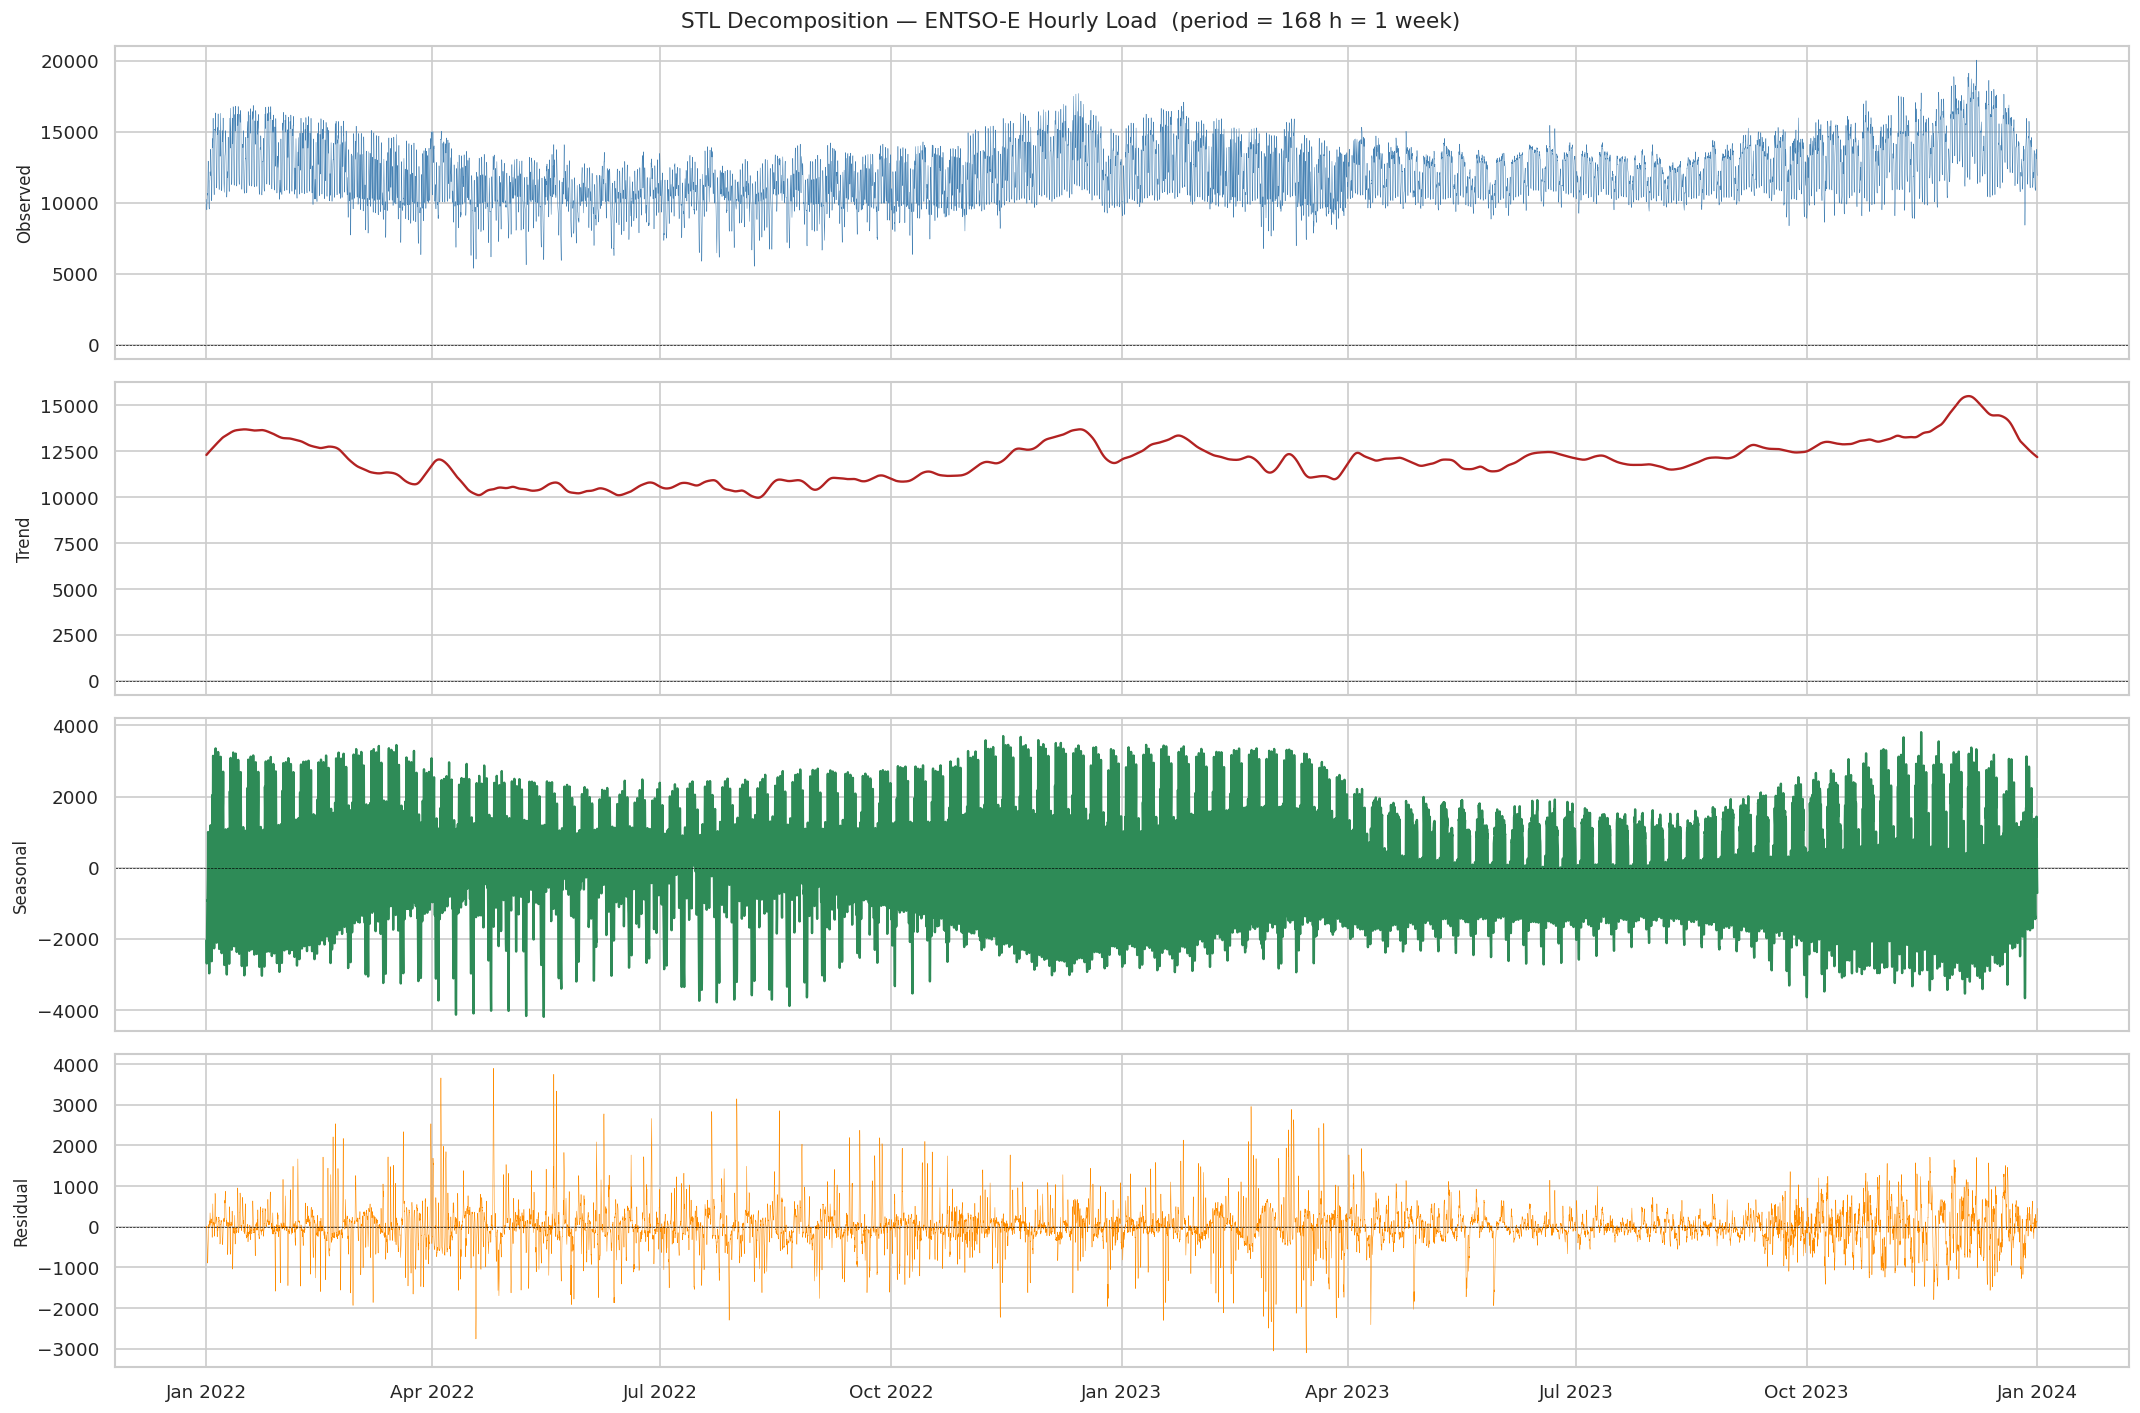
\includegraphics[width=\columnwidth]{figures/entsoe_02_stl.png}
    \caption{STL decomposition of ENTSO-E hourly electricity load (period $= 168$\,h). Seasonal variance dominates (58.0\%), with a visible 2022 demand trough in the trend component.}
    \label{fig:entsoe_stl}
\end{figure}

The autocorrelation function (ACF) confirms three dominant periodicities (Figure~\ref{fig:entsoe_acf}):

\begin{table}[htbp]
    \centering
    \caption{Top autocorrelation peaks of the ENTSO-E load series.}
    \label{tab:acf_peaks}
    \begin{tabular}{r r l}
        \toprule
        \textbf{Lag (h)} & \textbf{ACF} & \textbf{Interpretation} \\
        \midrule
        1 & 0.961 & Adjacent-hour persistence \\
        24 & 0.842 & Daily (diurnal) cycle \\
        168 & 0.924 & Weekly cycle \\
        \bottomrule
    \end{tabular}
\end{table}

\begin{figure}[htbp]
    \centering
    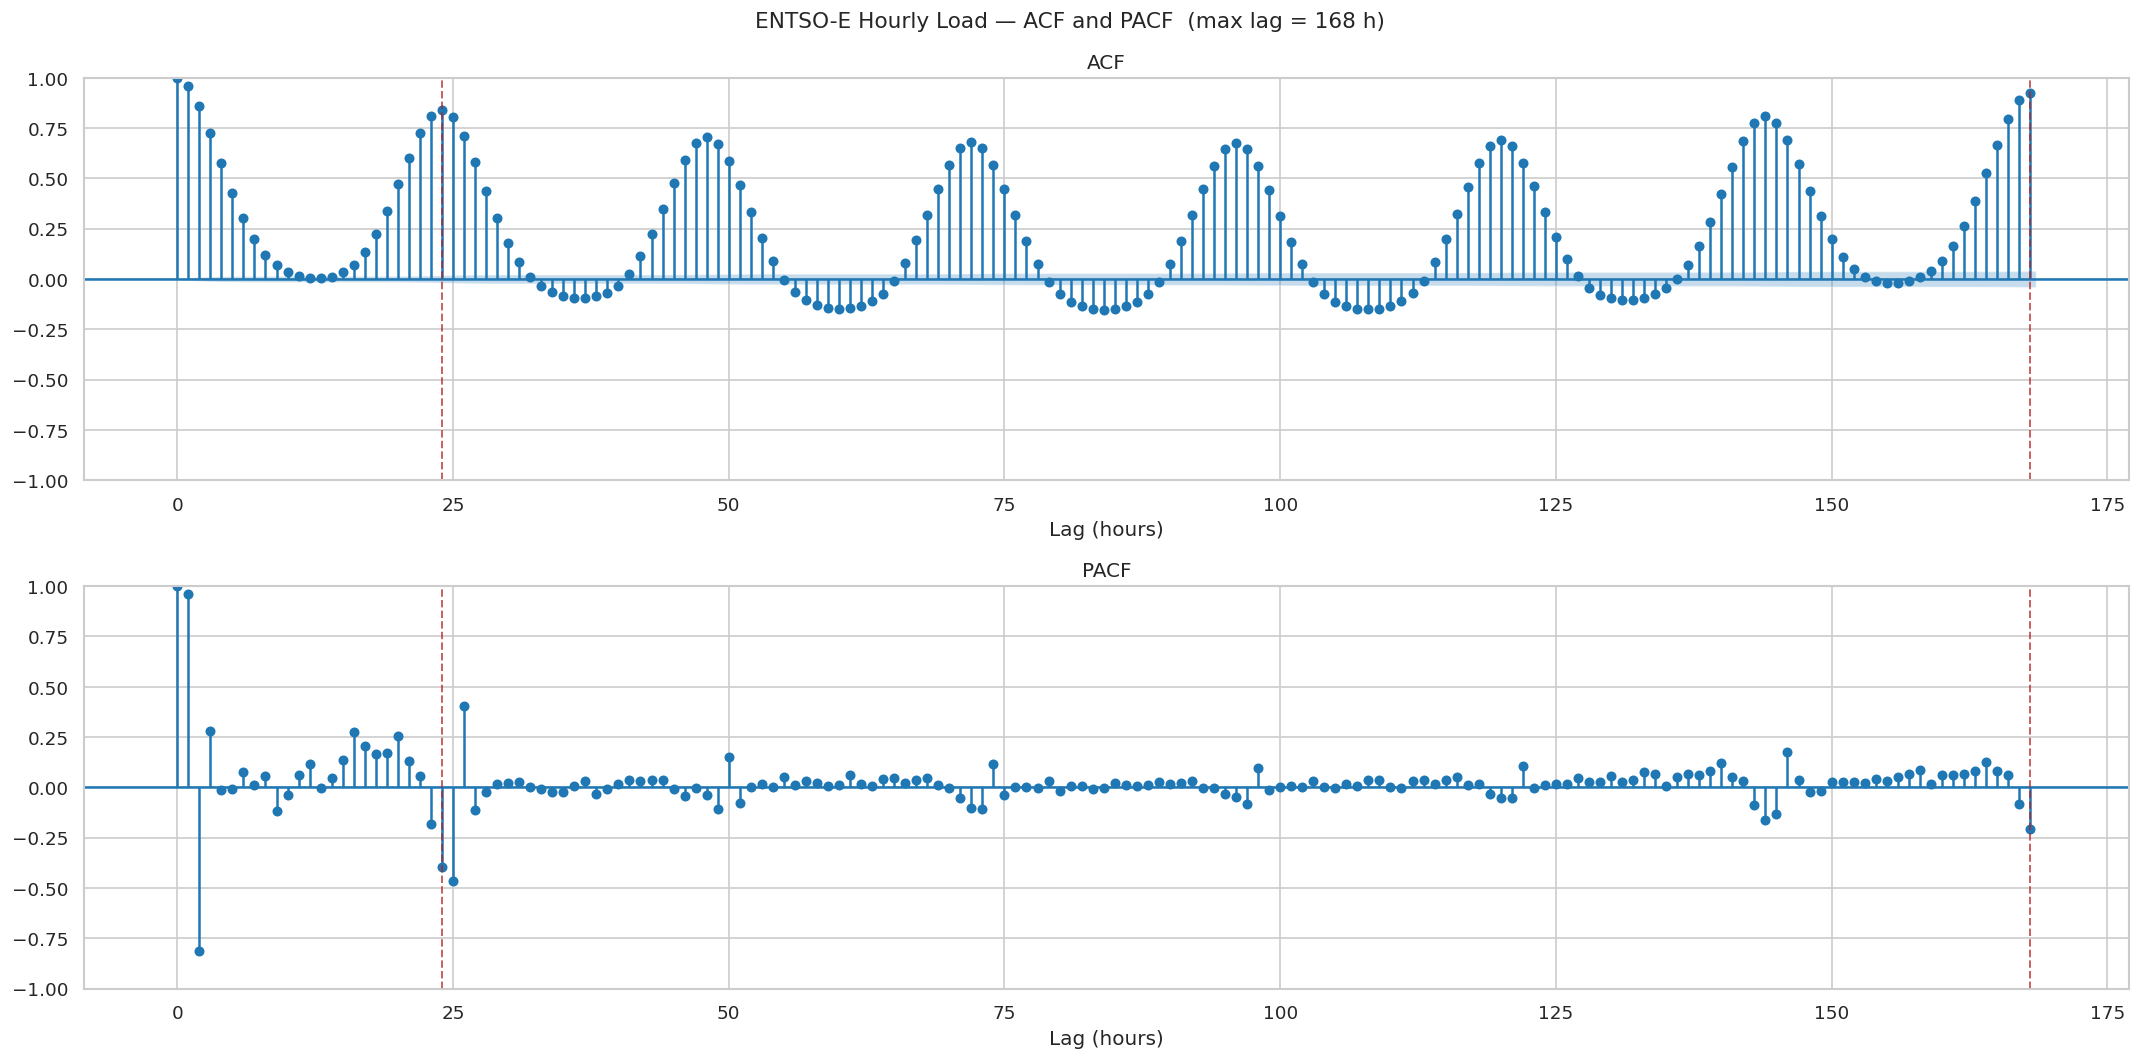
\includegraphics[width=\columnwidth]{figures/entsoe_03_acf_pacf.png}
    \caption{ACF and PACF of ENTSO-E hourly electricity load (168~lags). Strong peaks at lags 1, 24, and 168 confirm diurnal and weekly periodicity.}
    \label{fig:entsoe_acf}
\end{figure}

\noindent\textbf{Impact on design:} The dominance of the 24\,h and 168\,h cycles justifies the inclusion of explicit calendar features (\texttt{hour\_of\_day}, \texttt{day\_of\_week}, \texttt{month}) and autoregressive lag features at $t{-}1$, $t{-}24$, and $t{-}168$ (Section~\ref{subsec:feature_engineering}). The 2022 structural break motivates a binary energy-crisis indicator (Section~\ref{subsec:feature_engineering}). This aligns with the approach of Ashtar et~al.~\cite{ashtar_hybrid_2025}, who include a COVID-19 lockdown flag to capture analogous regime shifts.

\subsubsection{Weather--Load Relationship}
\label{subsubsec:eda_weather}

Among the KNMI validated meteorological variables, temperature exhibits the strongest contemporaneous correlation with load ($r = -0.178$; Figure~\ref{fig:weather_load}), confirming the Netherlands' heating-dominated demand profile: colder temperatures drive higher electricity consumption. Wind speed shows a weaker positive correlation ($r = +0.160$), likely reflecting wind-chill effects on heating demand. Humidity and solar radiation have near-zero contemporaneous correlations ($|r| < 0.03$).

\begin{figure}[htbp]
    \centering
    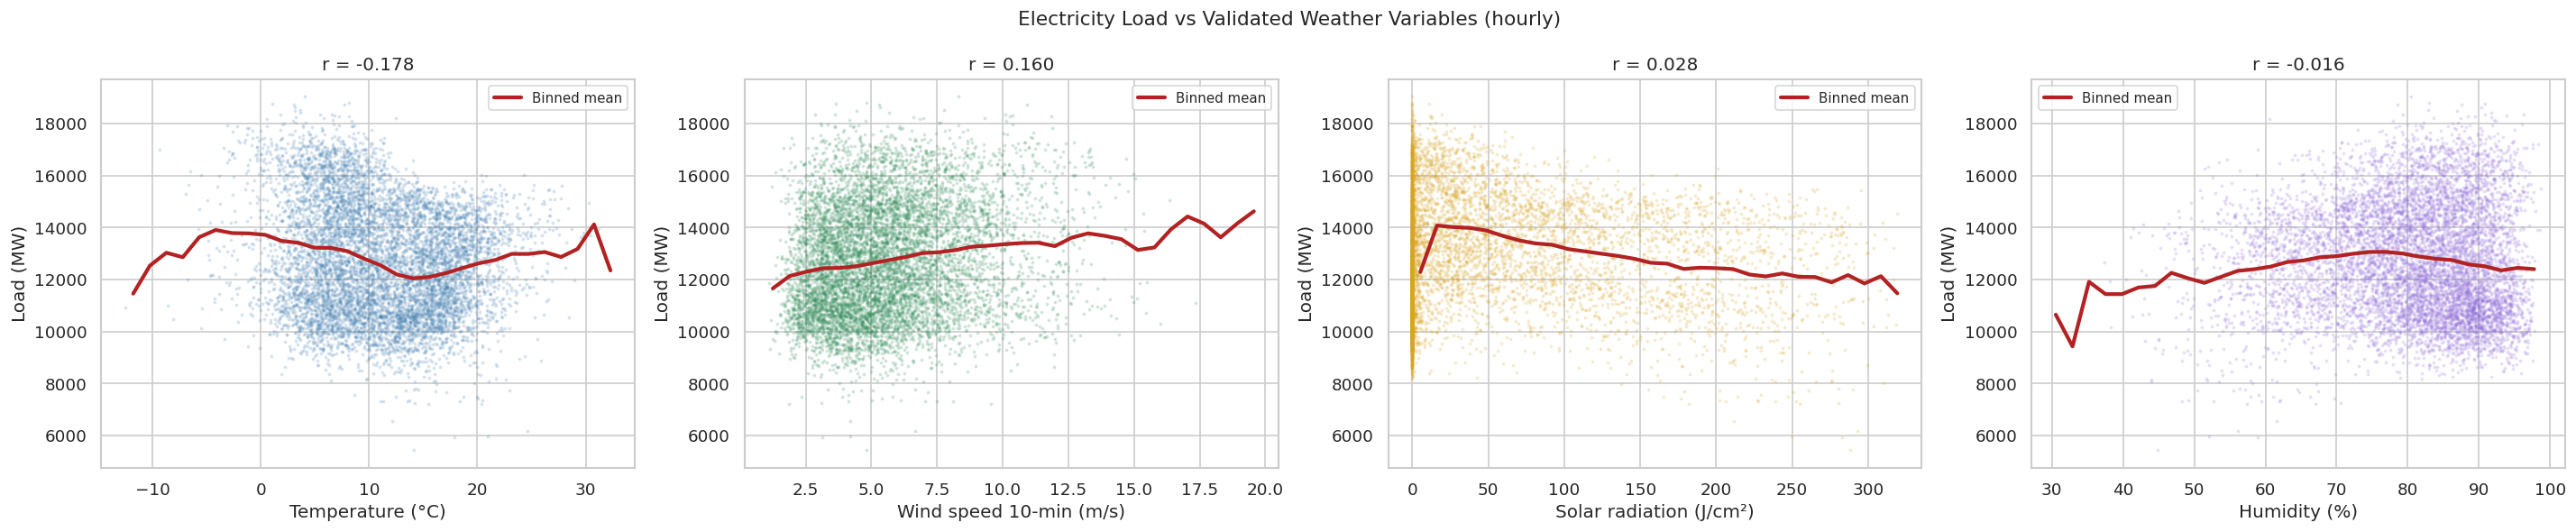
\includegraphics[width=\columnwidth]{figures/knmi_val_05_weather_load.png}
    \caption{Scatter plots of KNMI validated weather variables versus ENTSO-E load. Temperature shows the strongest negative correlation ($r = -0.178$).}
    \label{fig:weather_load}
\end{figure}

However, cross-correlation analysis (Figure~\ref{fig:ccf}) reveals that \textbf{solar radiation has the strongest \emph{lagged} relationship} with load: $r = -0.544$ at lag $+158$\,h (validated) and $r = -0.522$ at lag $-10$\,h (non-validated), versus near-zero at lag~0. This phase offset reflects the diurnal mismatch between peak solar generation (daytime) and peak grid demand (morning/evening), and the suppressive effect of photovoltaic generation on net load. Temperature peaks at $r = -0.410$ at lag $-83$\,h, capturing multi-day cold-spell persistence.

\begin{figure}[htbp]
    \centering
    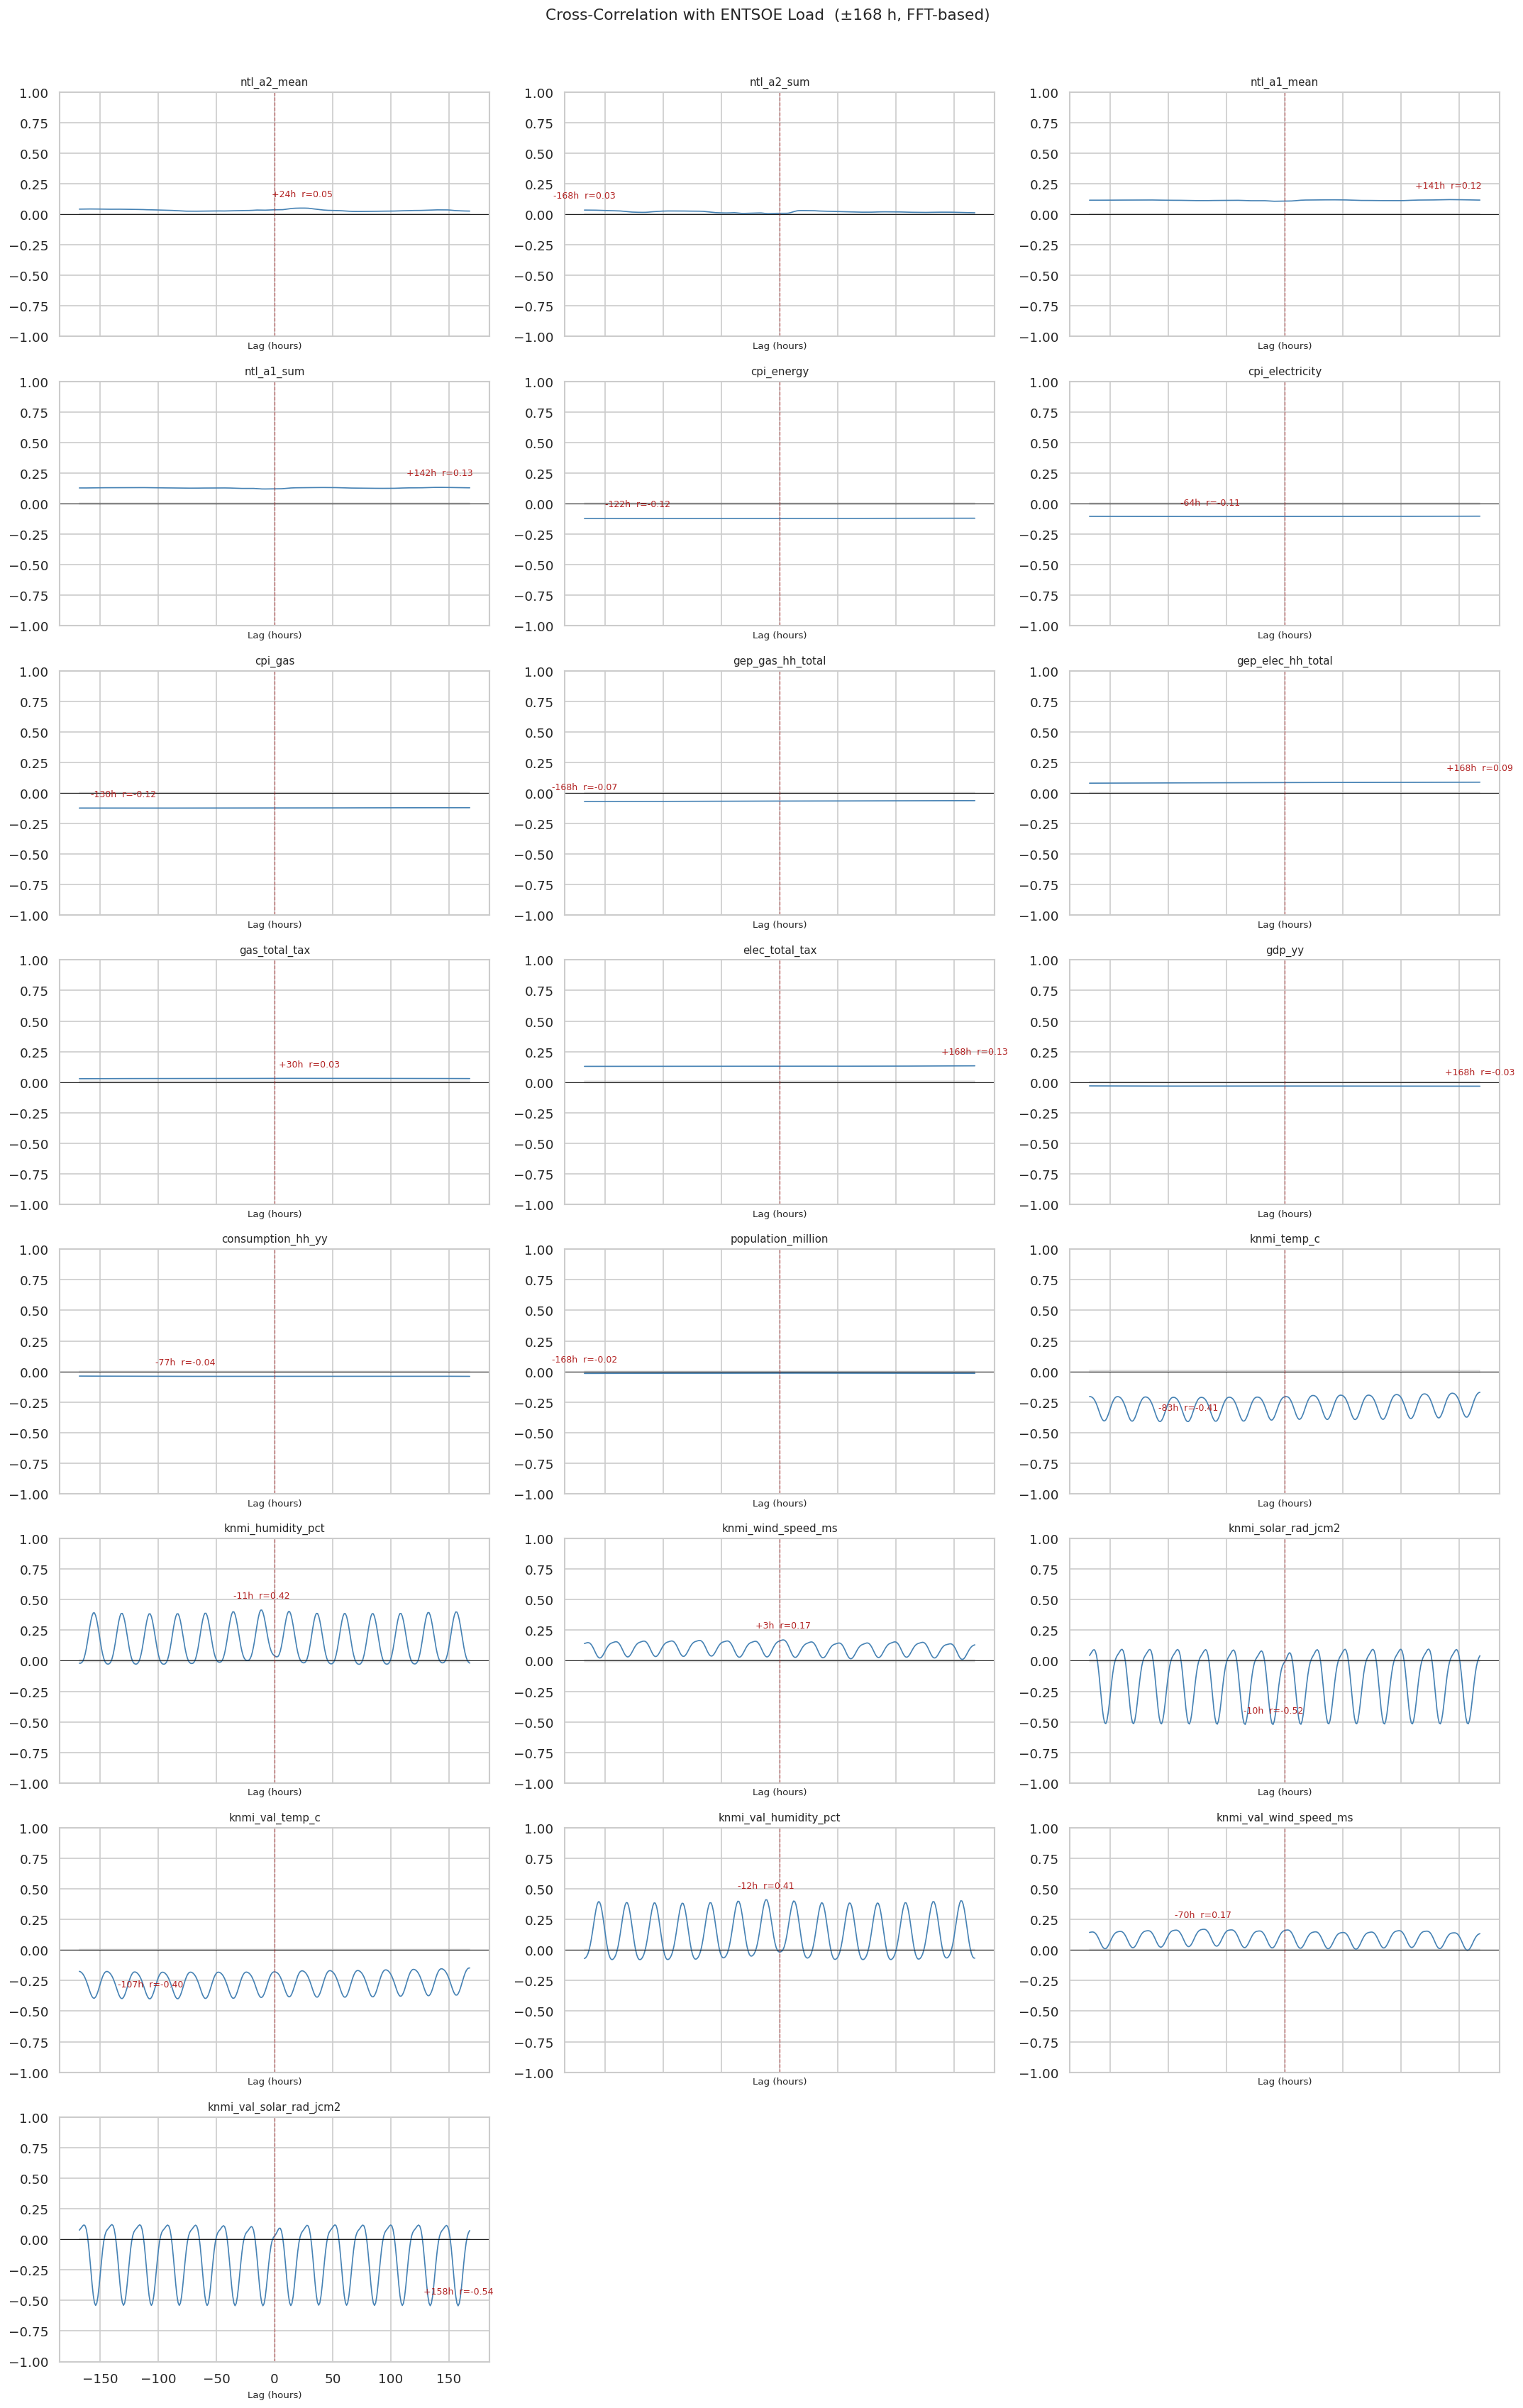
\includegraphics[width=\columnwidth]{figures/multi_03_ccf.png}
    \caption{Cross-correlation functions (CCF) between predictor variables and ENTSO-E load. Solar radiation achieves $r = -0.544$ at lag $+158$\,h; temperature achieves $r = -0.410$ at lag $-83$\,h.}
    \label{fig:ccf}
\end{figure}

\noindent\textbf{Impact on design:} The strong lagged solar-radiation signal motivates an explicit lagged solar feature (Section~\ref{subsec:feature_engineering}). This is analogous to the lag-based feature engineering in Ashtar et~al.~\cite{ashtar_hybrid_2025} and Curi\"el et~al.~\cite{curiel_integrating_2025}, who use rolling means and ACF-derived lags. Chen et~al.~\cite{chen_monthly_2025} instead model the temperature nonlinearity via a quadratic $T^2$ term and an NTL$\times T$ interaction, which is appropriate for their monthly granularity but unnecessary at hourly resolution where the temporal relationship can be captured via lags.

\subsubsection{NTL--Load Relationship and Survivorship Bias}
\label{subsubsec:eda_ntl}

The EDA revealed a critical finding regarding VIIRS product selection. The A2-selective product (quality~$\leq 1$ only) exhibits \textbf{severe survivorship bias}: the Netherlands' high cloud-cover rate ($\sim$52\textdegree N) causes the strict quality filter to admit only a tiny, non-representative subset of summer nights. In June, zero directly observed A2-selective pixels with $\geq$10\% spatial coverage exist across the entire 14-year record. The surviving clear-sky summer nights are drawn from anomalous anticyclonic high-pressure events, producing artificially elevated radiance values and a spurious summer peak that inverts the expected seasonal pattern.

\begin{table}[htbp]
    \centering
    \caption{NTL product comparison: correlation with ENTSO-E load and hourly coverage.}
    \label{tab:ntl_comparison}
    \begin{tabular}{l r r r}
        \toprule
        \textbf{Product} & \textbf{Coverage} & \textbf{Mean--load $r$} & \textbf{Sum--load $r$} \\
        \midrule
        VIIRS A1 & 96.4\% & $+0.108$ & $\mathbf{+0.121}$ \\
        VIIRS A2-all & 97.5\% & $+0.112$ & $+0.112$ \\
        VIIRS A2-selective & 54.7\% & $+0.037$ & $+0.008$ \\
        \bottomrule
    \end{tabular}
\end{table}

\noindent\textbf{Impact on design:} A2-selective is excluded from the feature set. \texttt{ntl\_a1\_sum} ($r = +0.121$) is adopted as the primary aggregated NTL feature, with \texttt{ntl\_a2\_all\_mean} as an ablation alternative. This contrasts with R.~et~al.~\cite{r_forecasting_2025}, who use A2 exclusively with quality~$\leq 1$ filtering; in their tropical Indian context, cloud contamination is less severe, and the survivorship bias is smaller. Our finding underscores that NTL product selection must be geography-specific.

Furthermore, the CCF analysis shows that \texttt{ntl\_a1\_sum} peaks at lag $+142$\,h ($r = 0.133$), not at lag~0 ($r = 0.121$). This confirms that NTL functions as a \textbf{multi-day economic-activity indicator} rather than an hourly load proxy, motivating its use as a slowly varying contextual signal in the cross-modal attention architecture rather than a direct hourly predictor.

\subsubsection{Multicollinearity}
\label{subsubsec:eda_vif}

Variance Inflation Factor (VIF) analysis on the full feature set reveals extreme multicollinearity (Figure~\ref{fig:vif}):

\begin{itemize}
    \item \texttt{ntl\_a1\_mean} and \texttt{ntl\_a1\_sum}: VIF $\approx 22.3 \times 10^9$ (near-perfect collinearity because A1's valid pixel count is nearly constant at 96.18\%, making $\text{sum} \approx \text{mean} \times 274{,}700$).
    \item KNMI humidity: VIF $> 50{,}000$ (correlated with temperature, solar radiation).
    \item CBS CPI energy/gas: VIF $> 9{,}000$ (pairwise $r = 0.990$).
    \item Validated vs.\ non-validated KNMI: pairwise $r > 0.99$ (near-duplicates).
\end{itemize}

\begin{figure}[htbp]
    \centering
    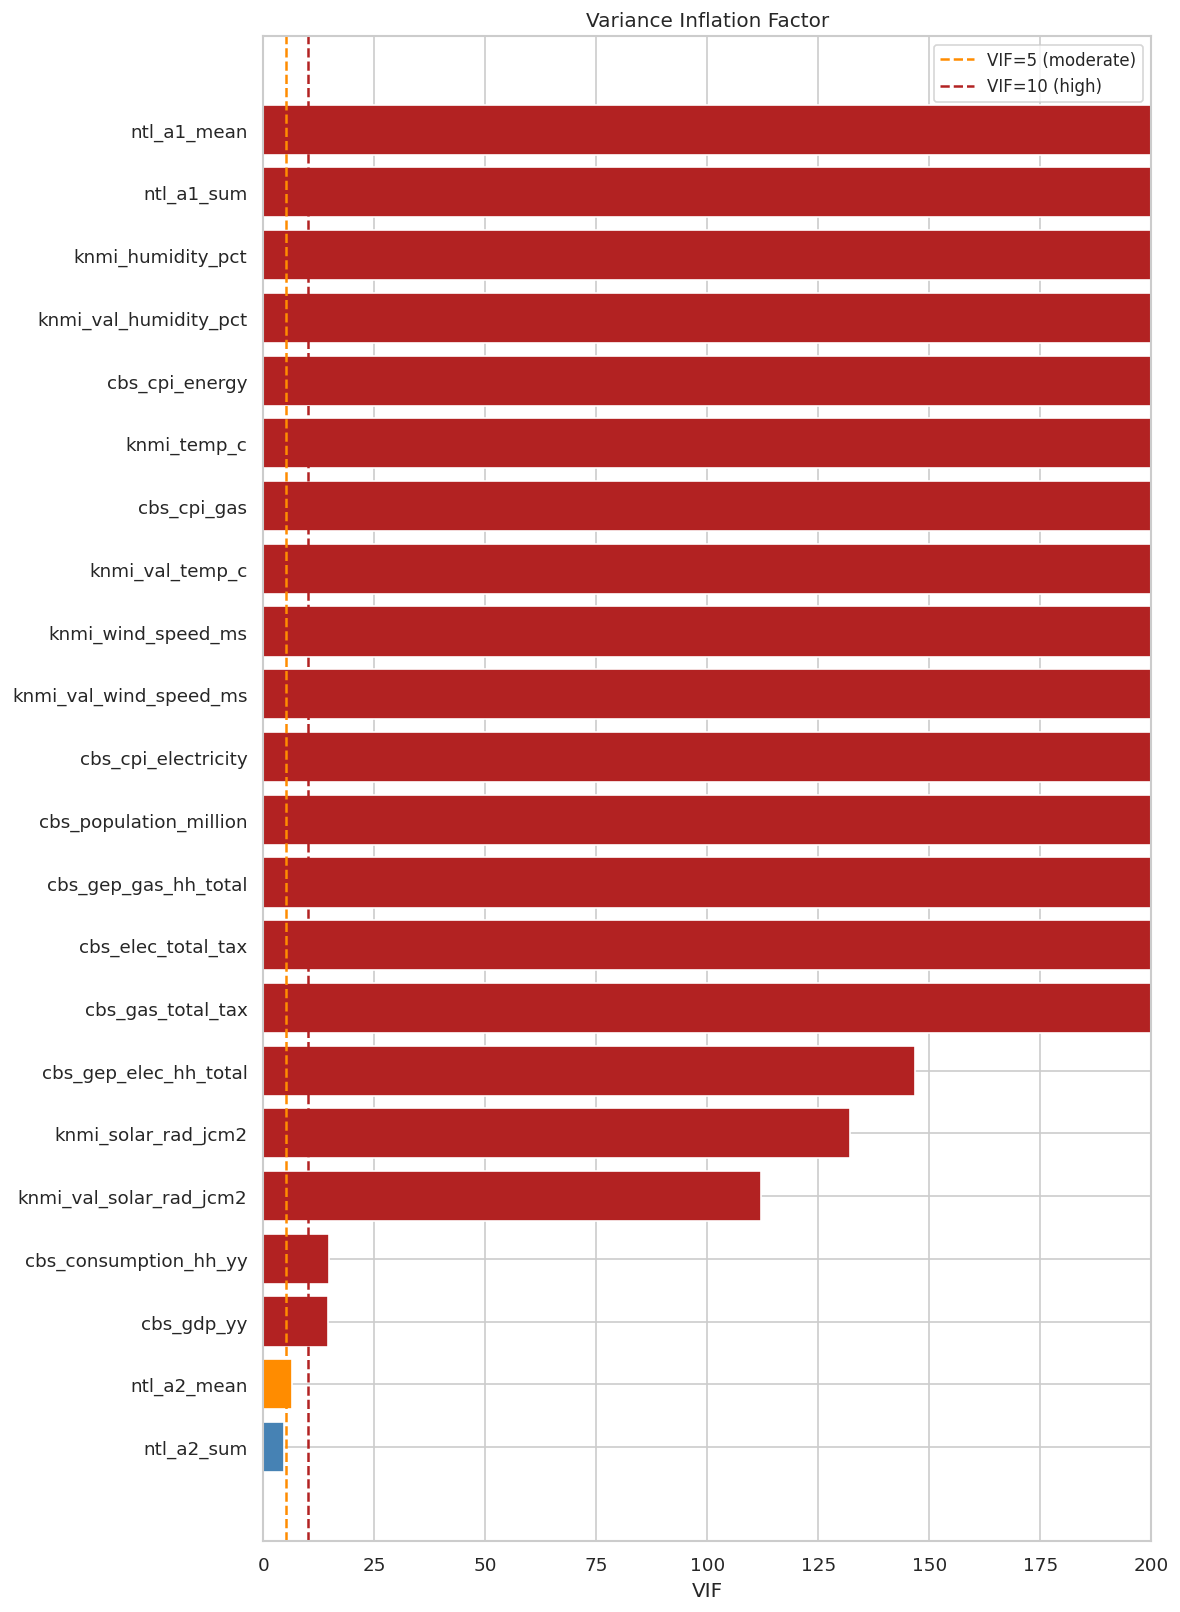
\includegraphics[width=\columnwidth]{figures/multi_02_vif.png}
    \caption{Variance Inflation Factors for the merged feature set. Several feature pairs exhibit extreme collinearity (VIF $> 10^4$).}
    \label{fig:vif}
\end{figure}

\noindent\textbf{Impact on design:} Aggressive feature pruning is required prior to model training (Section~\ref{subsec:feature_engineering}). Only one of \texttt{ntl\_a1\_mean}/\texttt{ntl\_a1\_sum} is retained; only the validated KNMI dataset is used; and a single CBS CPI variant replaces the collinear energy/gas/electricity trio. These VIF-driven decisions align with the multicollinearity analyses conducted by Ashtar et~al.~\cite{ashtar_hybrid_2025} and Curi\"el et~al.~\cite{curiel_integrating_2025} in their Dutch forecasting studies, though those studies did not need to address the satellite-specific collinearity issues arising from near-constant valid-pixel counts.

\subsubsection{CBS Economic Indicators}
\label{subsubsec:eda_cbs}

All CBS indicators are \textbf{trend-dominated}: CPI Energy 86.0\% trend variance, GEP Gas 90.9\%, GDP 55.8\%. They exhibit extreme persistence (ACF at lag~1: CPI Energy 0.970, GEP Gas 0.978) and capture slow macroeconomic shifts (energy-crisis price spikes, post-crisis recovery) rather than short-term demand fluctuations. This supports their role as contextual covariates processed through a dense FFN encoder (Section~\ref{subsec:models}) rather than as high-frequency predictors, consistent with the finding of Ashtar et~al.~\cite{ashtar_hybrid_2025} that socioeconomic indicators exhibit limited short-term predictive value for Dutch load.


%%%%%%%%%%%%%%%%%%%%%%%%%%%%%%%%%%%%%%%%%%%%%%%%%%%%%%%%%%%%%%%%%%%%%%%%%%%%%%%%
\subsection{Feature Engineering}
\label{subsec:feature_engineering}

This section describes the feature construction, selection, scaling, and missing-value treatment applied to the merged dataset prior to model training.

\subsubsection{Calendar and Temporal Features}
\label{subsubsec:calendar_features}

Explicit calendar encodings are derived from the UTC timestamp:

\begin{itemize}
    \item \texttt{hour\_of\_day} (0--23), \texttt{day\_of\_week} (0--6, Monday = 0), \texttt{month\_of\_year} (1--12), \texttt{week\_of\_year} (1--53), \texttt{quarter} (1--4), \texttt{day\_of\_year} (1--366).
    \item \texttt{is\_weekend} (binary): Saturday/Sunday.
    \item \texttt{is\_public\_holiday} (binary): Dutch national holidays (King's Day, Liberation Day, Christmas, New Year, Easter, Whit Monday, Ascension Day). These produce load dips of $\sim$2{,}000\,MW and are not derivable from date arithmetic alone.
    \item \texttt{is\_dst\_transition} (binary): Hours affected by daylight-saving-time clock changes.
\end{itemize}

The 24\,h (ACF = 0.842) and 168\,h (ACF = 0.924) autocorrelations confirm that calendar structure is the dominant signal in the target series (Section~\ref{subsec:eda}). Explicitly encoding these features substantially outperforms models that must learn temporal patterns from raw timestamps, as also demonstrated by Ashtar et~al.~\cite{ashtar_hybrid_2025}, who found that engineered temporal features were the single largest accuracy driver.

\subsubsection{Lag Features}
\label{subsubsec:lag_features}

Autoregressive lag features of the target variable are constructed at three horizons, justified by the ACF peaks identified in Section~\ref{subsubsec:eda_target}:

\begin{itemize}
    \item $y_{t-1}$: adjacent-hour persistence (ACF = 0.961).
    \item $y_{t-24}$: same hour yesterday (ACF = 0.842, diurnal cycle).
    \item $y_{t-168}$: same hour, same weekday, previous week (ACF = 0.924, weekly cycle).
\end{itemize}

These lag selections align with the feature engineering of Ashtar et~al.~\cite{ashtar_hybrid_2025}, who use previous hour/day/week lags, and Curi\"el et~al.~\cite{curiel_integrating_2025}, who include 24\,h, 7-day, and 12-month lags justified by identical ACF peaks. In contrast, R.~et~al.~\cite{r_forecasting_2025} rely on the LSTM's sequential input window (365~days for stacked/bidirectional variants) to implicitly capture lag structure, and Borunda et~al.~\cite{borunda_machine_2025} use 5~lagged annual NTL composites — a much coarser temporal approach justified by their annual forecasting horizon.

An explicit \textbf{lagged solar radiation feature} (\texttt{solar\_rad\_lag\_10h}) is constructed based on the CCF peak at lag $-10$\,h ($r = -0.522$; Section~\ref{subsubsec:eda_weather}). This captures the phase-delayed grid-demand suppression from daytime photovoltaic generation without requiring the model to learn the lag internally, following the general principle of Chen et~al.~\cite{chen_monthly_2025} who encode temperature nonlinearity explicitly rather than relying on the model to discover it.

\textbf{Note on lag availability:} All lag features use only past values ($t-k$, $k > 0$). At the start of the dataset (first 168~hours), lag values are unavailable and are set to \texttt{NaN}, which is handled by the missing-value treatment described below. For multi-step forecasting at horizon~$H_{\text{pred}}$, lag features at steps beyond $t+1$ would require predicted (not observed) past load. We adopt the \textbf{direct forecasting} strategy (one model per horizon) rather than recursive autoregression, sidestepping the issue of error accumulation in predicted lags.

\subsubsection{Step and Spike Variables}
\label{subsubsec:step_spike}

Two binary indicator variables are included to capture regime shifts identified in the EDA:

\begin{enumerate}
    \item \textbf{Energy-crisis flag} (\texttt{energy\_crisis}): set to 1 for the period 2022-01-01 to 2023-06-30, corresponding to the demand trough identified in Section~\ref{subsubsec:eda_target} (mean load 11{,}460\,MW in 2022 vs.\ 13{,}097\,MW in 2024). Without this indicator, a model trained on 2012--2025 will mis-learn the 2022 period as representative of normal demand levels. This is analogous to the COVID-19 lockdown flag used by Ashtar et~al.~\cite{ashtar_hybrid_2025}. Borunda et~al.~\cite{borunda_machine_2025} noted a similar COVID-19 structural break in Mexican consumption data (MAPE rising from 7\% to 34\% in 2020--2021) but opted not to model it explicitly, instead treating it as a limitation.

    \item \textbf{Public holiday flag} (\texttt{is\_public\_holiday}): captures the $\sim$2{,}000\,MW load dips on Dutch national holidays. Ashtar et~al.~\cite{ashtar_hybrid_2025} and Curi\"el et~al.~\cite{curiel_integrating_2025} handle holiday effects implicitly through Prophet decomposition components, while we encode them explicitly to ensure they are available to all model architectures including those that do not include a Prophet component.
\end{enumerate}

\subsubsection{Missing-Value Treatment}
\label{subsubsec:missing_values}

Missing values in the final dataset arise from three distinct mechanisms, each requiring a different treatment:

\begin{enumerate}
    \item \textbf{ENTSO-E load} (0.01\%, 13~hours): DST transition gaps. Filled by linear interpolation between adjacent hours.

    \item \textbf{NTL features} (2.5--3.6\% for A1/A2-all): genuine satellite orbit gaps and cloud-masked days. Filled by \textbf{forward-fill} from the most recent valid daily observation, reflecting the operational reality that at prediction time the most recent NTL image is the best available estimate. This is more conservative than the linear interpolation used by R.~et~al.~\cite{r_forecasting_2025} ($\text{SOL}_t = (\text{SOL}_{t-1} + \text{SOL}_{t+1})/2$), which requires future values and thus constitutes a minor form of data leakage.

    \item \textbf{CBS economic indicators} (0--43\%): null values arise from series starting after the dataset spine (e.g., CBS tariffs begin 2019). These are \emph{not imputed} but left as null, because the missingness is structural (data did not exist) rather than random. The model's macroeconomic encoder is designed to accept incomplete CBS feature vectors, replacing nulls with a learned default embedding. For the subset of CBS features with sporadic gaps within their coverage window, forward-fill is applied as described in Section~\ref{subsubsec:pipeline}.
\end{enumerate}

The thesis design originally proposed Multivariate Imputation by Chained Equations (MICE) for all missing data, following Curi\"el et~al.~\cite{curiel_integrating_2025} and Ashtar et~al.~\cite{ashtar_hybrid_2025}. However, the EDA revealed that the dominant missing-data patterns (NTL cloud gaps, CBS structural nulls) are \textbf{not Missing At Random (MAR)} — NTL missingness is strongly seasonal (cloud cover peaks in summer) and CBS missingness is deterministic (series start dates). MICE assumes MAR and would therefore introduce bias, particularly in NTL summer values where the surviving clear-sky nights are already non-representative (Section~\ref{subsubsec:eda_ntl}). We therefore adopt source-specific strategies as described above.

\subsubsection{Outlier Treatment}
\label{subsubsec:outliers}

The thesis design proposed Winsorization (percentile capping) for sensor outliers, following R.~et~al.~\cite{r_forecasting_2025}. The EDA did not reveal systematic outliers in the target variable or KNMI meteorological data that would warrant blanket Winsorization. The 2022 demand trough is a genuine structural shift, not an outlier, and is addressed via the energy-crisis indicator. VIIRS outliers (extreme radiance values from fires, gas flares, or sensor artefacts) are already handled upstream: the 10\% minimum coverage filter removes days with extreme spatial selection bias, and the quality-flag threshold ($\leq 1$) excludes fire-, cloud-, and snow-contaminated pixels. We therefore apply \textbf{no additional outlier removal} beyond the quality filtering already embedded in the ETL pipeline. This is more conservative than the IQR method of Curi\"el et~al.~\cite{curiel_integrating_2025} (applied to load in training folds only) or the Prophet-based anomaly detection of Chen et~al.~\cite{chen_monthly_2025}, but is justified by the absence of distributional anomalies in the EDA.

\subsubsection{Scaling}
\label{subsubsec:scaling}

All continuous features are normalised via \textbf{Min-Max scaling} to $[0, 1]$:
\begin{equation}
    \hat{x} = \frac{x - x_{\min}}{x_{\max} - x_{\min}}
\end{equation}
where $x_{\min}$ and $x_{\max}$ are computed \textbf{exclusively on the training fold} of each Rolling-Origin Cross-Validation split (Section~\ref{subsec:validation}), then applied to the corresponding validation and test folds. This prevents information leakage through scaling parameters, consistent with the protocol of Curi\"el et~al.~\cite{curiel_integrating_2025} and R.~et~al.~\cite{r_forecasting_2025}. Borunda et~al.~\cite{borunda_machine_2025} instead apply a natural-log transform; the choice of Min-Max over log-transform is motivated by the need for consistent scaling across heterogeneous feature types (MW, \textdegree C, nW/cm$^2$/sr, \%).

\subsubsection{Feature Selection Summary}
\label{subsubsec:feature_selection}

Based on the EDA findings (Section~\ref{subsec:eda}), the following feature-selection rules are applied to reduce the 114 raw columns to a curated predictor set:

\begin{enumerate}
    \item \textbf{Drop non-validated KNMI:} all \texttt{knmi\_*} columns (retain only \texttt{knmi\_val\_*}).
    \item \textbf{Drop A2-selective NTL:} \texttt{ntl\_a2\_mean}, \texttt{ntl\_a2\_sum} (survivorship bias; $r = +0.037$).
    \item \textbf{Drop \texttt{ntl\_a1\_mean}:} retain only \texttt{ntl\_a1\_sum} (VIF $\approx 22.3 \times 10^9$ between them; sum has higher $r$ with load).
    \item \textbf{Drop collinear CBS CPI:} retain \texttt{cbs\_cpi\_energy} only; drop \texttt{cbs\_cpi\_gas} ($r = 0.990$ with energy CPI) and \texttt{cbs\_cpi\_electricity}.
    \item \textbf{Drop \texttt{cbs\_gas\_total\_tax}:} collinear with \texttt{cbs\_population\_million} ($r = 0.973$).
    \item \textbf{Retain diagnostic pixel counts} (\texttt{ntl\_*\_valid\_count}, etc.) for quality-aware modelling but exclude from gradient-based optimisation.
\end{enumerate}


%%%%%%%%%%%%%%%%%%%%%%%%%%%%%%%%%%%%%%%%%%%%%%%%%%%%%%%%%%%%%%%%%%%%%%%%%%%%%%%%
\subsection{Models}
\label{subsec:models}

This section describes the proposed model architecture, the baseline models against which it is benchmarked, and the ablation study design. The proposed model is a Cross-Modal Attention Transformer (CMAT) adapted from the architectural principles of SolarCrossFormer~\cite{schubnel_solarcrossformer_2025} and the Causal-Aware Multimodal Transformer~\cite{wang_causal-aware_2025}.

\subsubsection{Baseline Models}
\label{subsubsec:baselines}

To isolate the value of VIIRS satellite imagery and cross-modal attention, the CMAT is benchmarked against established unimodal and hybrid models from the Dutch grid forecasting literature. All baselines are trained on identical temporal, meteorological, and economic data, completely omitting the VIIRS visual modality:

\begin{enumerate}
    \item \textbf{Prophet-LSTM}~\cite{van_de_sande_enhancing_2024}: Prophet learns trend, seasonality, and holiday effects; an LSTM learns non-linear residual dependencies. Achieved $r = 0.93$ and accurate forecasts up to 180~days.
    \item \textbf{SARIMAX-LSTM}~\cite{ashtar_hybrid_2025}: SARIMAX captures linear seasonal autoregressive structure; LSTM models residuals. Best-performing variant of the Ashtar et~al.\ study.
    \item \textbf{Sequence-to-sequence deep learning}~\cite{ashtar_hybrid_2025}: Encoder-decoder architecture with engineered temporal features. Achieved MAPE = 1.88\% at 180-day horizon.
    \item \textbf{XGBoost-stacked Prophet-LSTM and Prophet-QLSTM}~\cite{curiel_integrating_2025}: Two-stage stacking with XGBoost meta-learner. QLSTM achieved statistical parity with classical LSTM using $\sim$29$\times$ fewer recurrent parameters.
\end{enumerate}

The baselines span the major paradigms employed for this problem: decomposition-based hybrids (Prophet-LSTM, SARIMAX-LSTM), direct deep learning (Seq2Seq), and gradient-boosted stacking (XGBoost-stacked). This provides comprehensive coverage for benchmarking.

\subsubsection{Proposed Architecture: Cross-Modal Attention Transformer (CMAT)}
\label{subsubsec:cmat}

The CMAT processes three modality streams through dedicated encoders, fuses them via cross-modal attention, and decodes multi-step probabilistic forecasts.

\paragraph{Phase~1: Modality-specific feature projections.}
All modalities are projected into a shared latent dimensionality $d$ (search space: 32, 64, 128).

\begin{enumerate}
    \item \textbf{Temporal Transformer encoder.} The temporal inputs --- historical load, weather variables, calendar features, and lag features --- form a matrix $X_{ts} \in \mathbb{R}^{T \times F_{ts}}$, projected via linear mapping with learned temporal positional encoding. This is processed through $L$ layers of Multi-Head Self-Attention (MSA) with residual connections and layer normalisation, capturing autoregressive dependencies at the 1\,h, 24\,h, and 168\,h scales identified in the EDA.

    \item \textbf{Linear Patch Embedding (spatial encoder).} The VIIRS NTL satellite image $X_{img} \in \mathbb{R}^{C \times H \times W}$ (the most recent available A2-all daily composite; see revision in Section~\ref{subsec:data_preprocessing}) is divided into $N_p = \frac{H \times W}{P^2}$ non-overlapping patches of size $P \times P$, each flattened and linearly projected with spatial positional encoding. A shallow linear embedding is used instead of a full Vision Transformer (ViT) to prevent overfitting, following Schubnel et~al.~\cite{schubnel_solarcrossformer_2025}. Given that the effective independent sample size for the spatial modality is $\sim$4{,}950 unique daily images (A2-all at 97.5\% coverage, a revision upward from the thesis design's estimate of $\sim$4{,}748 based on A2-selective), the model-to-sample ratio must remain conservative.

    \item \textbf{Dense FFN encoder (macroeconomic context).} CBS macroeconomic indicators (GDP, CPI, population, tariffs) are aggregated into a static vector and processed via a dense Feed-Forward Network (FFN) into a single global contextual token. This is justified by the EDA finding (Section~\ref{subsubsec:eda_cbs}) that all CBS indicators are trend-dominated (86--91\% trend variance) with extreme persistence (ACF at lag~1 $> 0.91$), meaning they have negligible variance over the $\leq$2-week lookback windows used by the temporal encoder.
\end{enumerate}

\paragraph{Phase~2: Tripartite cross-modal attention.}
Visual and economic embeddings are concatenated along the sequence axis to form a unified exogenous context matrix $Z_{ctx} = [Z_{img} \parallel Z_{econ}] \in \mathbb{R}^{(N_p + 1) \times d}$. Cross-attention is computed with:
\begin{equation}
    \text{CrossAttn}(Q, K, V) = \text{softmax}\!\left(\frac{Q K^\top}{\sqrt{d}} + \mathcal{M}_{\text{mask}}\right) V
\end{equation}
where queries $Q$ are derived from the temporal sequence $Z_{ts}$ and keys $K$, values $V$ from the structural context $Z_{ctx}$. The causal mask $\mathcal{M}_{\text{mask}}$ prevents temporal tokens from attending to future time steps.

\paragraph{Phase~3: Factorised probabilistic decoder.}
The fused representation $Z_{\text{fused}} \in \mathbb{R}^{T \times d}$ is decoded via factorised linear projections:
\begin{equation}
    \hat{Y} = W_{\text{time}}^\top Z_{\text{fused}} W_{\text{quantiles}} \in \mathbb{R}^{H_{\text{pred}} \times 3}
\end{equation}
producing direct multi-step forecasts at three quantile levels $[\hat{y}_{0.05}, \hat{y}_{0.50}, \hat{y}_{0.95}]$, providing confidence intervals for grid operators as in Schubnel et~al.~\cite{schubnel_solarcrossformer_2025}. This avoids recursive autoregression and the associated error accumulation.

\paragraph{Regularisation.}
Given the model's estimated $\sim$300{,}000 trainable parameters against $\sim$4{,}950 effective visual samples, aggressive regularisation is essential:
\begin{itemize}
    \item \textbf{Dynamic image masking:} A random subset of satellite patch pixels is replaced with a learnable \texttt{[MASK]} token during training (masking rate: 0.50--0.95), as in~\cite{schubnel_solarcrossformer_2025}.
    \item \textbf{Time-series masking:} 10--15\% of past load and weather values are randomly masked, forcing cross-attention to query visual/economic modalities.
    \item \textbf{Architectural constraints:} 1--3 transformer layers, high dropout (0.2--0.4).
    \item \textbf{LR scheduling:} Cosine Annealing with Warm Restarts~\cite{schubnel_solarcrossformer_2025}, coupled with early stopping on the rolling-origin validation loss.
\end{itemize}

Hyperparameter optimisation is conducted via Bayesian optimisation over the search space in Table~\ref{tab:hyperparams}.

\begin{table}[htbp]
    \centering
    \caption{Hyperparameter search space for Bayesian optimisation.}
    \label{tab:hyperparams}
    \begin{tabular}{l l l}
        \toprule
        \textbf{Hyperparameter} & \textbf{Search Space} & \textbf{Rationale} \\
        \midrule
        Embedding dim.\ ($d$) & [32, 64, 128] & Constrains memorisation capacity \\
        Transformer depth ($L$) & [1, 2, 3] & Prevents spatial overfitting \\
        Lookback window ($T$) & [72h, 168h, 336h] & 168h captures weekly cycle \\
        Image masking rate & [0.50, 0.75, 0.95] & Extracts signal without memorising \\
        Dropout rate & [0.2, 0.3, 0.4] & Standard regularisation \\
        \bottomrule
    \end{tabular}
\end{table}

\subsubsection{Predictor Selection in the Full Model}
\label{subsubsec:predictor_selection}

The full CMAT model ingests the following predictor groups after feature engineering (Section~\ref{subsec:feature_engineering}):

\begin{enumerate}
    \item \textbf{Temporal encoder inputs:} lagged load ($y_{t-1}$, $y_{t-24}$, $y_{t-168}$), KNMI validated weather (temperature, wind speed, solar radiation, humidity, dew point), lagged solar radiation (\texttt{solar\_rad\_lag\_10h}), and all calendar/indicator features (hour, day-of-week, month, \texttt{is\_weekend}, \texttt{is\_public\_holiday}, \texttt{energy\_crisis}).
    \item \textbf{Spatial encoder input:} most recent A2-all daily NTL composite image (patch-embedded).
    \item \textbf{Macroeconomic encoder inputs:} \texttt{cbs\_cpi\_energy}, \texttt{cbs\_gdp\_yy}, \texttt{cbs\_population\_million}, \texttt{ntl\_a1\_sum} (as an aggregated economic-activity proxy), and selected GEP price variables.
\end{enumerate}

\subsubsection{Ablation Study Design}
\label{subsubsec:ablation}

Following the systematic ablation methodology of Wang et~al.~\cite{wang_causal-aware_2025}, five model configurations are trained and evaluated under the identical ROCV protocol (Section~\ref{subsec:validation}) to isolate the marginal contribution of each component:

\begin{enumerate}
    \item \textbf{TS Only:} Unimodal baseline using only load, weather, and calendar features (temporal encoder only, no cross-attention).
    \item \textbf{TS + Econ:} Bimodal; adds macroeconomic context. Cross-attention queries economic tokens only.
    \item \textbf{TS + Visual:} Bimodal; adds NTL imagery. Cross-attention queries image patches only.
    \item \textbf{Early Fusion:} All three modalities included via na\"ive concatenation into the temporal encoder input (cross-modal attention disabled). This isolates the contribution of the attention mechanism itself.
    \item \textbf{Full CMAT:} The complete architecture as described in Section~\ref{subsubsec:cmat}.
\end{enumerate}

The ablation enables quantification of three distinct contributions: (a)~the marginal value of NTL imagery (comparing configurations 1 vs.\ 3 and 2 vs.\ 5), (b)~the marginal value of cross-modal attention over na\"ive fusion (4 vs.\ 5), and (c)~the value of macroeconomic context (1 vs.\ 2). This mirrors the incremental component analysis of Wang et~al.~\cite{wang_causal-aware_2025} (text $\to$ image $\to$ cross-modal attention $\to$ adaptive weighting $\to$ causal discovery). A secondary ablation compares NTL product variants (\texttt{ntl\_a1\_sum} vs.\ \texttt{ntl\_a2\_all\_mean}) to validate the EDA-driven product selection.

Chen et~al.~\cite{chen_monthly_2025} perform a simpler ablation across 3-, 4-, and 5-parameter regression models, isolating the contribution of the NTL$\times T$ interaction and $T^2$ terms. Their approach is appropriate for their parametric regression framework but cannot capture the modality-level contributions that our transformer-based ablation is designed to measure. Borunda et~al.~\cite{borunda_machine_2025} similarly ablate by dropping predictors (NTL $\gg$ GDP $> T$), finding that NTL alone explains nearly all variance at annual/municipal granularity — a finding that motivates our inclusion of NTL but may not generalise to our hourly national-level setting.

\subsubsection{Optional Extension: Causal Discovery}
\label{subsubsec:causal_discovery}

To enhance interpretability, a secondary Causal Discovery Module based on the CAMT framework~\cite{wang_causal-aware_2025} may be integrated. This module applies Granger Causality principles via a sparsity-penalised network to learn a directed acyclic graph (DAG) of the features, enabling the model to attribute a predicted load change to specific causal drivers (e.g., a temperature drop, an economic shift, or a spatial NTL pattern change).


%%%%%%%%%%%%%%%%%%%%%%%%%%%%%%%%%%%%%%%%%%%%%%%%%%%%%%%%%%%%%%%%%%%%%%%%%%%%%%%%
\subsection{Validation and Evaluation Metrics}
\label{subsec:validation}

\subsubsection{Rolling-Origin Cross-Validation (ROCV)}
\label{subsubsec:rocv}

Because standard $k$-fold cross-validation induces severe data leakage in time-series data by allowing future observations to inform past predictions, we employ \textbf{Rolling-Origin Cross-Validation (ROCV)}, consistent with the protocols of Curi\"el et~al.~\cite{curiel_integrating_2025} (13-fold ROCV over 2010--2024) and Ashtar et~al.~\cite{ashtar_hybrid_2025}. In each fold $i$:

\begin{itemize}
    \item The training set comprises all data from the dataset start up to a rolling origin point $o_i$.
    \item The validation set spans the $H_{\text{pred}}$ hours immediately following $o_i$.
    \item The test set (for final evaluation) is held out entirely and never used for model selection.
\end{itemize}

The rolling origin advances in fixed increments (e.g., one month), producing an expanding training window that mimics the operational scenario where a grid operator re-trains or fine-tunes the model as new data arrives. Minimum training set size is 2~years ($\sim$17{,}520 hours), ensuring sufficient coverage of annual seasonality.

All preprocessing steps --- Min-Max scaling ($x_{\min}$, $x_{\max}$ computation), missing-value imputation parameters, and any feature-selection decisions --- are fitted \textbf{exclusively on the training fold} of each ROCV split and applied to the corresponding validation/test folds. This is consistent with the leakage-prevention protocols of Curi\"el et~al.~\cite{curiel_integrating_2025} (``MICE imputation and MinMaxScaling fitted strictly on training folds'') and R.~et~al.~\cite{r_forecasting_2025} (``chronological 80:20 split; scaling on train set only''). Borunda et~al.~\cite{borunda_machine_2025} use a simpler chronological 85/15 municipality-based split, which is appropriate for their cross-sectional setting but would be insufficient for our temporal forecasting task.

\subsubsection{Data Leakage Prevention}
\label{subsubsec:leakage}

Data leakage is prevented through multiple mechanisms:

\begin{enumerate}
    \item \textbf{Strict temporal ordering:} No future data is used in training. ROCV enforces $t_{\text{train}} < t_{\text{val}} < t_{\text{test}}$.
    \item \textbf{Training-fold-only preprocessing:} Scaling parameters and imputation statistics are computed on the training fold only (see above).
    \item \textbf{Forward-fill for low-frequency data:} CBS economic indicators are broadcast forward in time only, never backward (Section~\ref{subsubsec:pipeline}).
    \item \textbf{NTL forward-fill:} Missing NTL values are filled from the most recent \emph{past} observation, never interpolated with future values (unlike R.~et~al.~\cite{r_forecasting_2025}, who use bidirectional linear interpolation).
    \item \textbf{No contemporaneous exogenous inputs:} At prediction time $t$, only information available before $t$ is used (Section~\ref{subsec:problem_framing}). This distinguishes our approach from Chen et~al.~\cite{chen_monthly_2025}, who use same-month observed NTL and temperature.
\end{enumerate}

\subsubsection{Total Training Samples}
\label{subsubsec:training_samples}

The full dataset comprises 122{,}736 hourly records spanning 14~years (2012--2025). Using a sliding-window approach with hourly stride and a 168\,h lookback, the theoretical maximum number of training sequences is $\sim$122{,}500. However, the \textit{effective independent sample sizes} differ by modality:

\begin{itemize}
    \item \textbf{Temporal modality:} $\sim$122{,}500 unique hourly windows.
    \item \textbf{Spatial (NTL) modality:} $\sim$4{,}950 unique daily images (A2-all at 97.5\% coverage of 5{,}080~days). All 24~hourly windows within a given day share the same NTL image.
    \item \textbf{Economic modality:} $\sim$168 unique monthly CBS observations, repeated across all hours within each month.
\end{itemize}

The disparity between temporal ($\sim$122{,}500) and spatial ($\sim$4{,}950) effective sample sizes creates the overfitting risk described in Section~\ref{subsubsec:cmat}, motivating the aggressive regularisation strategy. With ROCV and a minimum 2-year training window, the first fold uses $\sim$17{,}500 hourly samples (corresponding to $\sim$730 unique NTL images); later folds use progressively more. This is substantially larger than the training sets of Chen et~al.~\cite{chen_monthly_2025} ($\sim$1{,}300 city-month samples), R.~et~al.~\cite{r_forecasting_2025} ($\sim$3{,}200 daily samples per LSTM), and Borunda et~al.~\cite{borunda_machine_2025} ($\sim$2{,}098 municipal cross-sections), providing a strong statistical foundation for training.

\subsubsection{Evaluation Metrics}
\label{subsubsec:metrics}

Model performance is evaluated using a multi-metric approach to capture different facets of predictive accuracy, enabling direct comparison with prior Dutch studies:

\begin{enumerate}
    \item \textbf{Root Mean Square Error (RMSE):}
    \begin{equation}
        \text{RMSE} = \sqrt{\frac{1}{n} \sum_{i=1}^{n} (y_i - \hat{y}_i)^2}
    \end{equation}
    Penalises large errors disproportionately; the primary metric for Wang et~al.~\cite{wang_causal-aware_2025} (12.3\% reduction reported).

    \item \textbf{Mean Absolute Percentage Error (MAPE):}
    \begin{equation}
        \text{MAPE} = \frac{100}{n} \sum_{i=1}^{n} \left| \frac{y_i - \hat{y}_i}{y_i} \right|
    \end{equation}
    Enables comparison with Ashtar et~al.~\cite{ashtar_hybrid_2025} (1.88\% at 180~days) and Borunda et~al.~\cite{borunda_machine_2025} (7\% average MAPE).

    \item \textbf{Mean Absolute Error (MAE):}
    \begin{equation}
        \text{MAE} = \frac{1}{n} \sum_{i=1}^{n} |y_i - \hat{y}_i|
    \end{equation}
    Robust to outliers; reported by R.~et~al.~\cite{r_forecasting_2025} and Borunda et~al.~\cite{borunda_machine_2025}.

    \item \textbf{Pearson Correlation Coefficient ($r$):}
    Captures the linear association between predicted and actual load. Enables comparison with van~de~Sande et~al.~\cite{van_de_sande_enhancing_2024} ($r = 0.93$) and Borunda et~al.~\cite{borunda_machine_2025} ($R^2 > 0.85$).
\end{enumerate}

For probabilistic forecasts (quantile outputs), the \textbf{Pinball Loss} (Quantile Regression Loss) is additionally computed:
\begin{equation}
    \mathcal{L}_{\tau}(y, \hat{y}) = \begin{cases}
        \tau (y - \hat{y}) & \text{if } y - \hat{y} \ge 0 \\
        (\tau - 1)(y - \hat{y}) & \text{otherwise}
    \end{cases}
\end{equation}
for $\tau \in \{0.05, 0.50, 0.95\}$. This is the training objective for the CMAT and provides operationally useful prediction intervals. Schubnel et~al.~\cite{schubnel_solarcrossformer_2025} demonstrate the practical value of probabilistic forecasts for grid operators in the solar-irradiance domain; we adopt the same paradigm for load.

All metrics are reported separately for each forecasting horizon ($H_{\text{pred}} \in \{168, 720, 1{,}440\}$\,h) and each ROCV fold, with fold-aggregated means and standard deviations providing confidence estimates. Statistical significance between model pairs is assessed via the Wilcoxon signed-rank test on fold-level metrics, following R.~et~al.~\cite{r_forecasting_2025}.
